% %This is a very basic article template.
% %There is just one section and two subsections.
\documentclass{scrartcl}

\usepackage[ colorlinks=true, urlcolor=blue, linkcolor=green ]{hyperref}
\usepackage[title]{appendix}
\usepackage{graphicx}

\begin{document}

\title{Evaluation of Domain-Specific Languages in Practice\\}
\subtitle{Proposal for a Habilitation at the Technische Universit\"at M\"unchen}

\author{Dr. Levi L\'ucio}

\maketitle

\abstract{In this document we introduce our research topic of interest for
pursuing a habilitation at theTechnische Universit\"at M\"unchen.}

\section{Document Structure}

We will start by providing some background about the topic of Domain-Specific
Languages in section~\ref{sec:background}. We then go in
section~\ref{sec:soa} on to discuss the state of the art of the domain and to
highlight the trends in the domain. In section~\ref{sec:topic} we introduce our
topic of interest and in section~\ref{sec:context4dev} we lay out the context
under which the research will take place.

\section{Background}
\label{sec:background}

Computer languages are very often domain-specific, in the sense that they
specialize in describing specifications, operational or not, of certain
artifacts. Domain-Specific Languages (DSLs) are often presented in opposition ro
General-Purpose Languages (GPLs) which are all-purpose generic programming
languages such as Java or C. The premise of DSL construction is that such
languages should explicitly address a domain of interest by making the concepts
of the domain first-class citizens~\cite{Kolovos06}. This can imply a trade-off
in generality, meaning some DSLs may not be Turing-complete as such
computational power may not be required in the domain of interest. The
advantages put forward by the proponents of the DLS approach are increased
productivity for language users and reduced maintenance costs of DSL programs.
Additionally, DSLs are expected to lower the barrier of computer language usage
to non-experts, thus allowing users from other domains to more easily specify
the artifacts and computations they require~\cite{MernikHS05}.

DSLs have a rich history of contributions in different areas of knowledge.
Notable examples of DSLs that left permanent marks in their domains are
\emph{lex} and \emph{yacc}~\cite{Johnson80} for compiler construction,
HTML~\cite{BernersLee96} for the world-wide web, VHDL~\cite{Ashenden02} for
hardware specification, Excel for spreadsheets, Latex~\cite{Lamport1989} for
typesetting, SQL~\cite{Codd70} for database querying or MATLAB~\cite{Gilat07}
for technical computing.

During the past decade a number of DSL workbenches saw the light of day. The
Eclipse Modelling Framework (EMF) had significant impact in the academia and
became one of the most popular frameworks for DSL construction. More recently,
the MPS workbench from Jetbrains has delivered a powerful DSL construction
workbench with professional support and possibilities to design attractive GUIs
that provide a very interesting complement to the notion of domain specificity.
Professional DSL workbenches such as MetaEdit+ have repeatedly made strong cases
for the industrial adoption of DSLs and have gathered a niche market in the
domain.

During the past few years, DSLs have attracted considerable interest from the
industry. The paradigm speaks directly to engineers who wish to build their
systems ground-up and making as much use as possible of domain knowledge that is
typically hard-earned. In this context, clients often regard DSLs as key-in-hand
solutions. They encompass simplified means to express domain-specific
computations while abstracting from accidental complexity linked to the software or the hardware
running underneath.

Companies such as itemis, PROTOS or MetaCase have successfully developed
business models around DSLs. They leverage their knowledge of modelling and DSL workbenches to
deliver to customers key-in-hand software solutions. Such solutions have been
developed for disparate domains such as the automotive, avionics, power tools,
health, biology, among many others, and help either software developers or final
users in achieving their tasks.

Despite these successes, the potential and real impact of DSLs in industry is
still ill understood. A recent compelling report from Tolvanen and
Kelly~\cite{Tolvanen016} states that while their company specialized in
DSLs, MetaCase, can affirm with certainty that the gains in productivity of
their clients range from 500\% to 1000\%. In the same article, they claim
academic research in the domain thus not been able to validate this in general.
They speculate this is due on the one hand to the quality of their tool
MetaEdit+ and their industrial experience, and on the other hand to the poor
quality of the academic tools for supporting DSL construction.

Anecdotally, at the PAINS workshop at MODELS 2018, an interesting discussion
raged between a high-profile DSL proponent and a top-level BMW manager. While
the DSL proponent insisted that the (MPS-based) technology was ready and could
serve as a ``silver bullet'' of sorts, the BMW manager replied that the attempts of using
DSLs at his company where ``hit-and-miss'' and that even when DSLs did prove
successful, it was not understood why. A question from that same manager that
was particularly thought-provoking was: ``how do I build and abstraction and
know that it is a good one?''. A more general criticism to the DSL approach in
general was: ``quality standards are missing, how do I to judge or trust your
processes of building DSLs while making decisions that will benefit my company?''.
 
\section{State of the Art}
\label{sec:soa}

In 2000, a landmark white paper from the company MetaCase
claimed that, using their commercial tool MetaEdit+, they developed DSLs that 
increased the productivity of the company 10-fold~\cite{metacase00}. Such claims
spawned a large amount of interest both in the industry and academia for DSLs.

Following such interest, authors such as Spinellis or V\"olter pursued the idea
of proposing patterns for DSLs construction~\cite{Spinellis01,VolterB04}, much
in the light of what had been very successfully done by the ``gang of four'' for
design patterns~\cite{Gamma:95}. Such research culminated in the very well-cited
work of Mernik, Heering and Sloane in 2005~\cite{MernikHS05} which builds on
the work of Spinellis and aims at providing the DSL developer with the
understanding of where and when design decisions matter in DSL development.
Also, reports on industrial best practices such as the work from
Wile~\cite{Wile03} started to emerge at this time.

The raise in interest also brought upon a number of DSL workbenches both
open-source and commercial such as the Eclipse Modelling Framework
(EMF) for Eclipse~\cite{emf} or Microsoft's DSL tools~\cite{microsoftDSLTools},
GME~\cite{gme} or AToM3~\cite{atom3}. In particular, EMF was heavily adopted by
academia for pursuing research on DSLs and together with GMF~\cite{gmf} soon
became the platform of choice for academic DSL development.
 
While the enthusiasm around DSLs continued strong throughout the 00s and work on
how to develop good languages kept on being published~\cite{Voelter09}, other
authors began to question the state of practice in general. In particular Kelly
from MetaCase raises in~\cite{Kelly2009} the point that DSL development often
takes a standpoint of self sufficiency, ignoring pitfalls that mostly have to do
with taking the domain for which the language is developed or its users too
lightly. This was in the same year corroborated by work from Gabriel \emph{et
al.}~\cite{Gabriel09} who reviewed a significant amount of literature related to
the evaluation of DSLs. The authors claim that, while the benefits of DSLs in
terms of increased productivity in well-defined domains were often put forward
in the literature, little to no evidence to back up such claims was offered.

Having recognized the fact that DSLs were critically missing supporting
evaluation that would back up the promises from the early days, authors such as
Kolovos and Paige~\cite{Kolovos06} proposed sets of characteristics that
``good'' DSLs should exhibit. Examples of such generic characteristics are
conformity to the domain of choice, supportability by tools, integrability with
other languages, longevity, simplicity, quality, scalability or usability.
Several studies from the late 00's and beginning of the 10's~\cite{Kolovos06}
have concentrated on proposing means to quantitatively assess such
and other
characteristics~\cite{KellyTolvanen09,Hermans09,Barisic:12,Kahraman2015}. A
notable study dating from this period from Kosar \emph{et al.}~\cite{Kosar2012}
provides empirical evidence that programs written using DSLs are more easily
comprehensible by programmers than programs written using GPLs, one of the
original claims of the DSL community.

During this same period several contemporary DSL workbenches made their first
appearance: the Meta Programming System (MPS)\footnote{Note that while the MPS
project exists since 2003, its mainstream appearance dates to a decade later.}
from JetBrains~\cite{mps}, Sirius used by Obeo as a core
technology~\cite{sirius}, Xtext from itemis AG~\cite{xtext}, among
others~\cite{Kelly:2013}. Benefiting from the previous decade of development
and professional software development teams, these tools exhibit a level of
maturity that allows them to be used in industrial settings with success. For instance Sirius has been used to develop
DSLs for the aerospace, transportation or energy industries~\cite{obeo}.
MPS~\cite{mps} has been used to develop commercial tools for branches such as
software development, health, financial companies or automotive, among others.
Xtext~\cite{xtext} is also used by large players such as Google, SAP or Bosch.

While the above seems to indicate that DSLs have successfully permeated the
industry, authors from recent surveys remain very critical of the actual state
of the art. Mernik~\cite{Mernik17} published a systematic mapping study in
2017 where he shows that the \emph{maintenance} and \emph{validation} phases of
DSL development are grossly under-studied in the literature when compared to the
\emph{domain analysis}, \emph{design} and \emph{implementation} phases (see
figure~\ref{fig:DSL_design_phases}).

\begin{figure}[!h]
\centering 
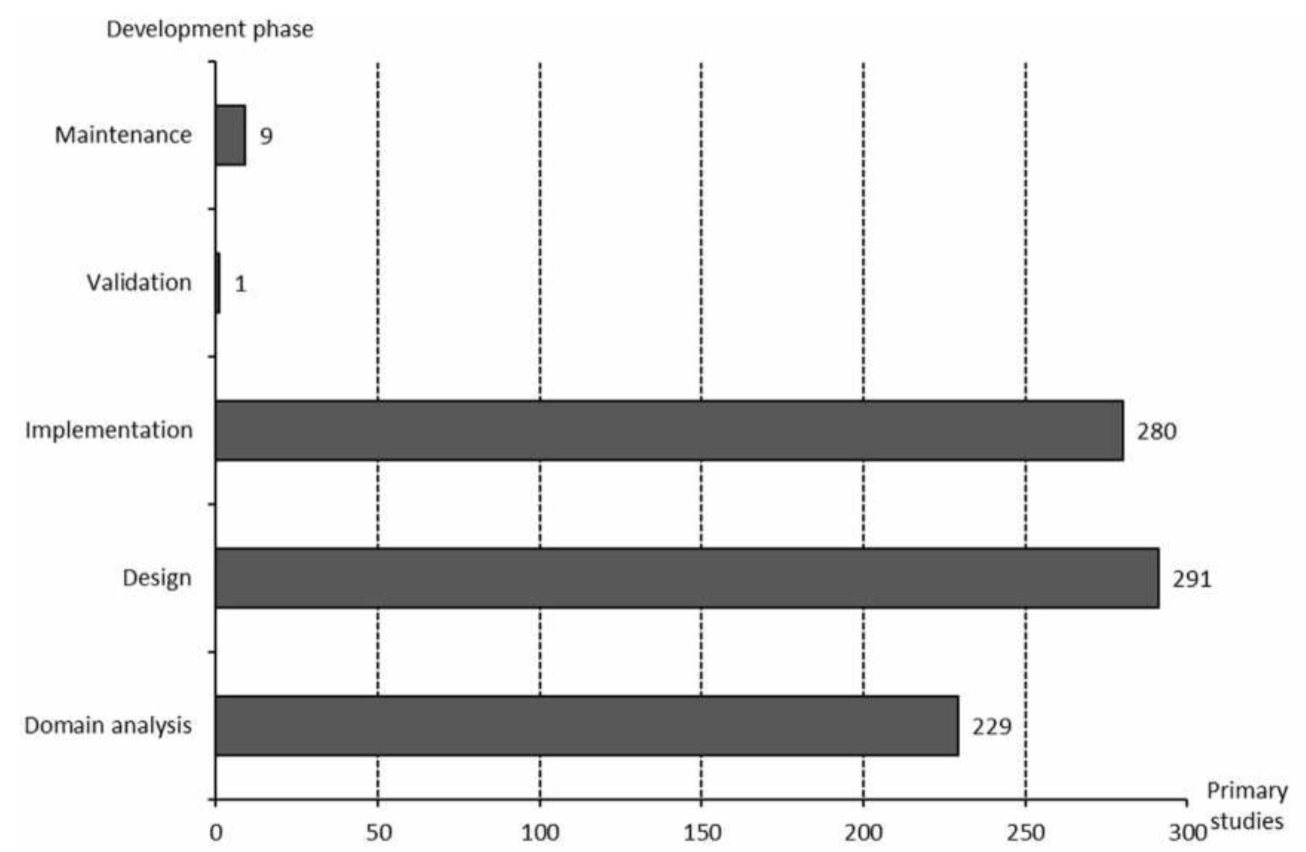
\includegraphics[width=1\textwidth]{./figures/DSL_design_phases}
\caption{Distribution of 810 scientific contributions by phases of DSL
construction (extracted from~\cite{Mernik17})}
\label{fig:DSL_design_phases}
\end{figure}

Equally, Tolvanen and Kelly who have been active DSL community since the late
90's have recently published a summary of their experiences with their
commencial tool MetaEdit+~\cite{TolvanenKelly2016}. There, they state that
although they can consistently claim a 5 to 10 times improvement in productivity
for their customers, the DSL community has not been able to do the same in
general. Note that this does not contradict the paragraph above on adoption by
the industry, as: 1) adoption does not mean increased productivity, and 2) it is
to be expected that if productivity increases do exist, corporate secrecy would
be used to avoid losing competitive advantages. Tolvanen and Kelly do mention
in~\cite{TolvanenKelly2016} that the reason why the academic community has
failed so far to prove or disprove most of the fundamental claims for advantages
of DSLs is the poor quality of the overall tooling as well as DSLs used and
developed by academic research. This notion is shared by us.

Nonetheless, modern DSL workbenches have provided the means for experimenting
with the construction of DSLs in a systematic manner. Based on the work of
Freire \emph{et al.}~\cite{Freire14} on formalizing software engineering
experiments, H\"aser and his colleagues have proposed in~\cite{Haser16} a
framework in MPS that allow defining and conducting experiments for validating
DSLs. Very recently work has started to emerge on concrete frameworks for the
evaluation of usability during DSL development~\cite{Barisic18} and DSL
maintenance~\cite{ThanhoferPilisch17} -- responding to the issues identified by
Mernik~\cite{Mernik17} illustrated in figure~\ref{fig:DSL_design_phases}.

\paragraph{Summary}
From the state of the art above, we can identify the following tends:

\begin{itemize}
  \item For almost two decades professional DSL workbench builders have
  consistently reported case studies of application of DSLs to industrial
  problems, some of those use cases being highly successful.
  They do nonetheless mention that obtaining the data for validating the DSL
  after shipment is hard~\cite{Tolvanen018}.
  \item During that same period academia as struggled to provide evidence that
  the promises of DSLs in terms of increased productivity hold. Only recently,
  partly due to the arrival of mature DSL workbenches produced by professional
  software, is actual quantification of properties of DSLs such as e.g.
  usability becoming possible. Experimental validation of DSLs based on
  established theory is still under-explored~\cite{Mernik17}.
  \item The DSL workbenches developed by academia are, thus far, insufficient to
  scientifically validate the premises of the DSL-based software development.
  This is due partly to the poor quality of the tooling
  produced by academia~\cite{TolvanenKelly2016} and partly to very low access to
  real industrial use cases. Most of the surveys we describe above use as study
  material other academic papers, leading to starvation of real information
  ``from the trenches''.
  \item With the notable exceptions of the work of Tolvanen and Kelly and
  Völter mentioned above in this section, the bridges between the academia and
  industry are brittle in the DSL domain.
\end{itemize}

\section{Proposed Topic of Research}
\label{sec:topic}

From the state of the art in section~\ref{sec:soa} it is clear to us that a
substantial gap exists between academic research in DSLs and their usage in
practice. For this reason, we formulate our main research question as:\\

\textbf{How can we identify, measure and use characteristics of DSLs that lead
to their sustained and sustainable adoption by the industry?}\\

Such a research naturally leads to a number of sub-research questions, namely:

\begin{itemize}
  \item What are the characteristics of a DSL that can be quantitatively
  assessed in order improve the chances of a real increase in productivity by
  the industry?
  \item What tooling is adequate to do such quantitative assessment?
  \item How can those characteristics be summarized in a way that is convincing
  for software-agnostic staff (domain experts or management), leading to the
  qualification of the DSL development process?
\end{itemize}

Regarding the tooling used to perform the quantitative assessment, we are firmly
convinced that areas such as formal methods and machine learning have an
important role to play and we have collected evidence of this through our past
work (see section ~\ref{sec:context4dev}). We thus formulate a corollary
research questions as: how can formal methods and machine learning help
in the qualification and production phases of a DSL?

Note that our mid-to-longterm goal is to inseminate the academic community with
the practical experiences and struggles of making DSLs used practice, leading
to the theoretical establishment of the domain.

\section{Context for Development of the Research}
\label{sec:context4dev}

We have significant experience in the design and implementation of DSLs for
areas such as software testing~\cite{lucio08}, model
transformations~\cite{BarrocaLAFS10}, verification~\cite{OakesTLW15,kanav18},
process management~\cite{LucioARAKH17} and software refinement~\cite{Syriani19}. Such
languages were also developed over a variety of DSL workbenches, for instance
the Eclipse EMP framework, MPS or AToM3. Some of the DSLs were developed for
academic purposes, while other were or are being developed with industrial
partners such as Diehl Aerospace, Airbus and Rolls-Royce.
 
The role that fortiss itself plays and will play on this research is not to be
understated: at fortiss we have built and currently have the kind of access to
projects and industrial and academic partners that occurs very seldom in academia.

Not to be understated also is the existing body of research on the topic we are
proposing. Although the gap between academia and industry is clear and has been
repeatedly stated in the literature we have reviewed in section~\ref{sec:soa},
exciting results on validating DSLs such as the ones recently presented
by Lara \emph{et al.}~\cite{LaraGuerra13}, Freire \emph{et al.}~\cite{Freire14}, 
Haser \emph{et al.}~\cite{Haser16} or Barisic \emph{et al.}~\cite{Barisic:12}
are starting points for this research. Also, systematic work by
Mernik~\cite{MernikHS05, Kosar2012, Mernik17} on assessing the state of the art
provides an excellent starting point for this research, as well as the clear-cut
reports from the industry from Kelly and Tolvanen~\cite{Tolvanen016, Kelly2009,
KellyTolvanen09, Kelly:2013, TolvanenKelly2016, Tolvanen018} and
V\"olter~\cite{Voelter09}.

!!!something on FM and ML here!!!

In the annexes of this document we provide detailed information about the
context in which our research will be developed:

\begin{itemize}
  \item Synergies with groups at fortiss (appendix~\ref{app:synergies})
  \item Completed and running projects at fortiss (appendix~\ref{app:projects})
  \item Network (appendix~\ref{app:network})
  \item Objectives for the first year of research (appendix~\ref{app:first_year_objectives})
\end{itemize}

\pagebreak
 
\begin{appendices}

\section{Synergies with groups at fortiss}
\label{app:synergies}

Domain-Specific Languages are a cross-cutting theme at fortiss. All
competence fields at fortiss deal with DSLs in one form or the
other, even or despite doing it unknowingly.

\begin{itemize}
\item The obvious synergy of our research topic is with the Model-Based
Software engineering (MbSE) group:
MbSE has a model-centric view on systems and software engineering and builds languages using model-driven
techniques. Its main current theme is design-space exploration and the modelling
of  embedded systems, but other themes such as requirements engineering, formal
methods or security are also being pursued. DSLs can be of great assistance to
MbSE by bringing systematic notions of language construction and evaluation to
the development table. A collaboration that is already ongoing is the
exploration of machine learning (in the context of the MAGNET project) to deliver support to users of AF3.
\item Common work is also ongoing with the Autonomous Systems (AS) group, in the
form of the FaktorBUILD project proposal. Some of the work of AS relies on probabilistic
programming to model situations where incomplete knowledge must be reliably used
to make decisions in real-time. Here, we help in constructing DSLs at an
adequate level of abstraction such that the IDE provided to users of factor
graphs can leverage good abstractions, static analyses and formal methods to
increase the productivity of factor graph programmers.
\item The collaboration with the Industry 4.0 (i4) group has been so far very
successful, having lead to the implementation of a tool
providing DSLs to express industrial capabilities. Such capabilities, or
skills, can be subsequently be matched to automatically automatically synthesize
controllers for industrial machines. Upcoming work for 2019 in the area will aim
at connecting the completed DSL-based tool to AutomationML and 4Diac in order
to connect the work with outside formats while providing simulation capabilities. 
\end{itemize}

\section{Completed and Running Projects at fortiss}
\label{app:projects}

\begin{itemize}
  \item IETS3
  \begin{itemize}
    \item Consortium: fortiss, itemis, ZF, Diehl aerospace
    \item Running time, funding and personnel: 2 years / ~300K Euro / 3 people
  \end{itemize}
\end{itemize}

\begin{itemize}
  \item CBMD (as project leader)
  \begin{itemize}
    \item Consortium: fortiss, PROTOS, SQMi, University of Augsburg
    \item Running time, funding and personnel: 2 years / ~190K Euro / 2 people
  \end{itemize} 
  \item MAGIC (as project leader)
  \begin{itemize}
    \item Consortium: fortiss, University of Montréal
    \item Running time and funding: 2 years / ~10K Euro + ~40K Euro
    (Eigenforshungsgeld) / 3 people
  \end{itemize} 
  \item MAGNET (as project leader)
  \begin{itemize}
    \item Consortium: fortiss
    \item Running time, funding and personnel: 6 months / ~70K Euro / 8 people
    Eigenforshungsgeld
  \end{itemize}
  \item ARTEMIS (as project leader)
  \begin{itemize}
    \item Consortium: fortiss, Airbus
    \item Running time, funding and personnel: 6 months / 75KEuro / 2 people
    (Levi + HiWi)
  \end{itemize} 
  \item BaSys4.0 (as software developer for the ``industrial skills'' theme )
\end{itemize}

\section{Network}
\label{app:network}

Here I will describe the main currently active research and industrial
connections (others exist that may be reactivated at need):\\\\
\textbf{Inside fortiss:}

\begin{itemize}
  \item HCE (Yuanting Liu and team, project MAGNET)
  \item SD (Tahira Iqbal and Parisa Elahidoost, project MAGNET and requirements
  engineering)
  \item i4 (project MAGIC, networking with University of Montréal)
  \item AS (Dhiraj Gulati and Vincent Aravantinos, on BaSys and FactorBUILD)\\
\end{itemize}
\textbf{Academic}:

\begin{itemize}
  \item University of Montr\'eal, Canada (project MAGIC)
  \item University of Namur, Belgium (tutorial and paper on machine learning and
  formal verification)
  \item University of Antwerp, Belgium (proposal for H2020)
  \item LMU, Germany (with Prof. Dirk Beyer in the context of the FaktorBUILD
  proposal)
  \item University of L\"ubeck, Germany (with Prof. Philipp Rostalski in the
  context of the FactorGraph proposal)
  \item TU Wien (with Manuel Wimmer in the context of model transformations)\\
\end{itemize}
\textbf{Industrial:}

\begin{itemize}
  \item PROTOS (KMU) (in the context of the CBMD project)
  \item Rolls-Royce (in the context of the EARS-related work)
  \item Siemens (in the context of the FaktorBUILD proposal)
  \item Festo (in the context of the BaSys project)
  \item ABB (in the context of the BaSys project)
\end{itemize}

\section{Objectives for the first year of research}
\label{app:first_year_objectives} 

\begin{itemize}
  \item Establish a set of criteria for the quality of DSLs in practice. In
  particular, we are interested in understanding which measurable criteria can
  be used to facilitate the adoption of DSLs in the industry.
  \item Evaluate the usage of machine learning in the context of requirements
  engineering and in general as a means to aid in the construction and operation
  of good and reliable DSLs.
  \item Establish an ongoing collaboration with Prof. Dirk Beyer from the LMU in
  Munich. Prof. Beyer is an expert in formal methods and is part of the
  consortium for the FaktorBUILD project. He is, in particular, very
  enthusiastic about applying his CPAchecker C model checker to examples coming
  from Airbus Defense in the context of the ARTEMIS project. Publishing with
  Prof. Beyer will also be pursued.
  \item Evaluate the prototype developed for the MAGNET project in the
  real-world scenario of tutorials of AF3. Calibrate the suggestions provided by
  the machine learning algorithm in function of such an evaluation.
  \item Write one or more articles on the results of the MAGNET project.
  \item Evaluate the usage of machine learning in the context of requirements
  engineering and in general as a means to aid in the construction and operation
  of good and reliable DSLs.
\item Establish a set of criteria for the quality of DSLs in practice. In
particular, I am interested in understanding which measurable criteria can be used to
facilitate the adoption of DSLs in the industry.
  \item Write one or more articles on the results of the skills (F\"ahigkeiten)
  work-package of the BaSys project.
 \item Continue research on the topic of Process-Aware model driven development
environments to be implemented in AF3. Complete the ongoing journal paper on
process-aware model-driven development environments.
 \item Help Sudeep Kanav in establishing his PhD research topic by publishing
 results on compositional model checking at top venues. Continue Sudeep's
 scientific training.
 \item Provide Tatiana Chuprina with the right tools such that she can finish
 her thesis proposal in the area of requirements engineering.
\end{itemize}

\subsection{Technical:}

\begin{itemize}
  \item Build a prototype tool in MPS to generate LTL from EARS requirements and
  model-check C code written for those requirements. 
  \item Build a release-ready prototype of a recommender system for AutoFOCUS3
  that can be effectively used in tutorials on the tool given to industry or
  academia.
  \item Complete the development of the skill-matching and controller
  synthesis prototype for BaSys. The prototype will semi-automatically generate
  a controller for a robotic arm in 4Diac. A demonstrator of the complete chain
  from skill definition down to robot arm movement will be built based on
  virtual robotic arm simulator provided by Festo AG. 
  \item Integrate compositional model checking in the eTrice tool, such that it
  can be used in production by PROTOS.
\end{itemize}

\end{appendices}

\bibliographystyle{plain}
\bibliography{group_proposal}

\end{document}
 